\subsection{Получение информации о команде c помощью команды whatis и apropos}

\subparagraph{1) Что нужно было сделать?}

Получить краткую информацию по командам ls и cd с помощью команды whatis и apropos. В чем различие?

\subparagraph{2) Как это сделали?}

\begin{MyVerbatimCode}[label=Debian terminal]
pavel-innokentevich-galanin@aspire-one-725:~$ whatis ls
ls (1)               - list directory contents
pavel-innokentevich-galanin@aspire-one-725:~$ whatis cd
cd: nothing appropriate.
\end{MyVerbatimCode}

\begin{figure}[!htp]
    \begin{minipage}{0.49\textwidth}
        \centering
        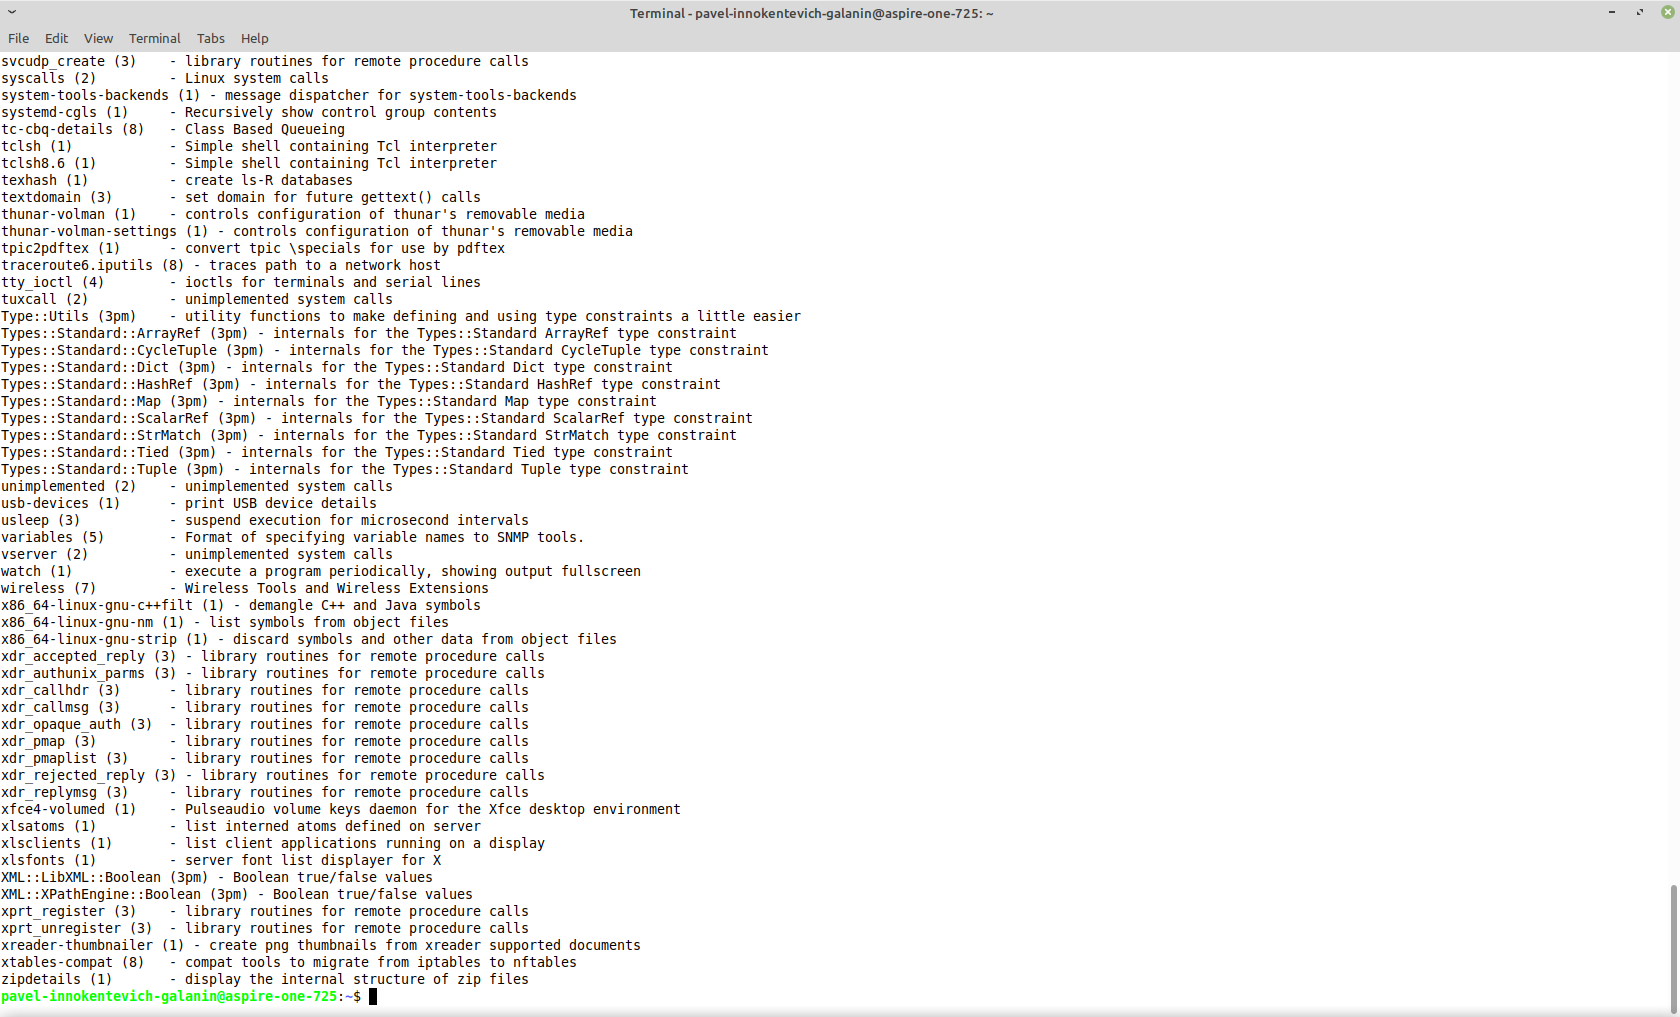
\includegraphics[width=\linewidth]
            {input/task-1/6/apropos-ls.png}
        \caption{apropos ls}
        \label{fig:apropos-ls}
    \end{minipage}
    \begin{minipage}{0.49\textwidth}
        \centering
        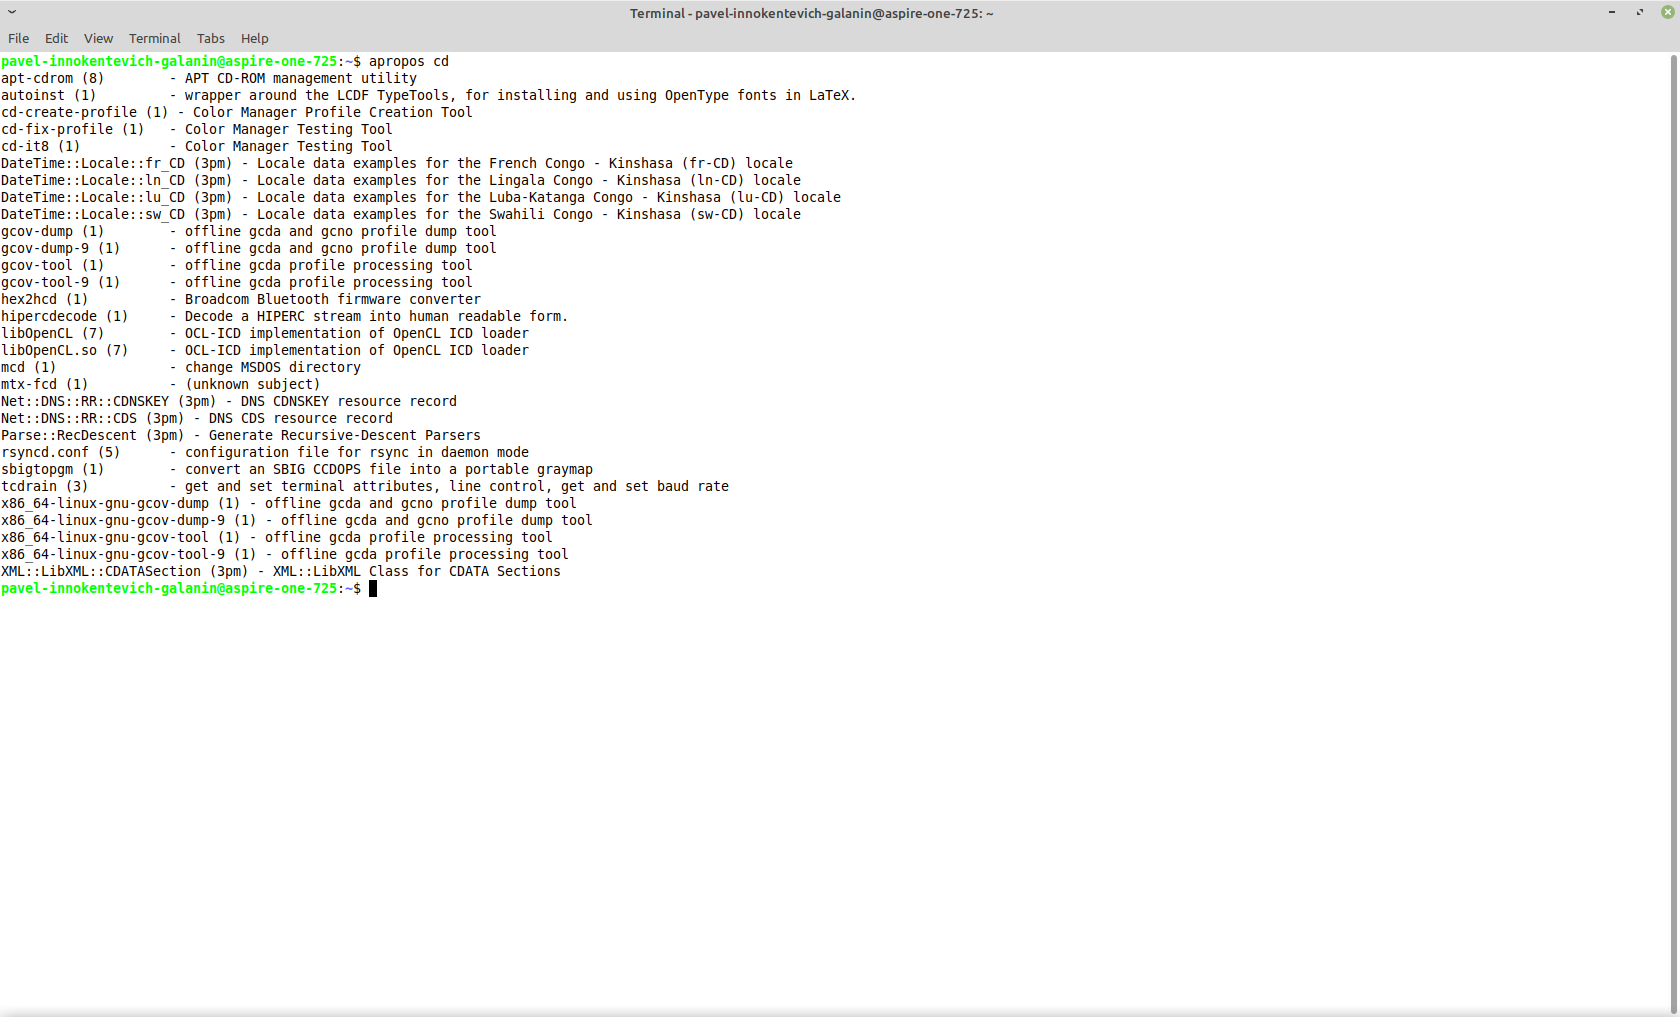
\includegraphics[width=\linewidth]
            {input/task-1/6/apropos-cd.png}
        \caption{apropos cd}
        \label{fig:apropos-cd}
    \end{minipage}
\end{figure}

Результат выполнения команды apropos ls
на~рисунке~\ref{fig:apropos-ls}
(стр.~\pageref{fig:apropos-ls}).

Результат выполнения команды apropos cd
на~рисунке~\ref{fig:apropos-cd}
(стр.~\pageref{fig:apropos-cd}).

\subparagraph{3) Что получилось?}

Командой whatis получили в консоль краткую инфомарцию о введённой команде, если справки нет, то выводится сообщение об отсутсвии. Командой apropos получили подробный справочный вывод в консоль о введённой нами команде.
